\section{EXPERIMENTS}
\begin{table*}
\caption{Performance of the \eks and \uks methods compared to their GP counterparts (\egp and \ugp) on a range of synthetic benchmarks. 
\gp is the corresponds to the GP analytical solution in the linear case.
}
\begin{center}
\begin{tabular}{c c c c c}
g(f) & Method & SMSE-f* (std) & NLPD-f* (std) &SMSE-g* (std) \\ 
\toprule
linear & \eks & 0.0441 (0.0100) & -0.8671 (0.0884) & 0.0440 (0.0099) \\ 
& \uks & 0.0441 (0.0100) & -0.8670 (0.0883) & 0.0440 (0.0098) \\ 

& \egp & 0.0324 (0.0146) & -1.0105 (0.2995) & 0.0324 (0.0146) \\ 
& \ugp & 0.0345 (0.0176) & -0.9392 (0.4295) & 0.0345 (0.0176) \\ 

poly3 & \eks & 0.0332 (0.0274) & -0.7883 (1.2629) & 0.0096 (0.0074) \\ 
& \uks & 0.0697 (0.0311) & 0.9693 (1.3725) & 0.0173 (0.0067) \\ 

& \egp & 0.0671 (0.0247) & -0.3596 (0.6799) & 0.0164 (0.0053) \\ 
& \ugp & 0.0579 (0.0360) & -0.3544 (0.6156) & 0.0138 (0.0085) \\ 

exp & \eks & 0.0360 (0.0322) & -0.9672 (0.7705) & 0.0171 (0.0131) \\ 
& \uks & 0.0230 (0.0071) & -1.2456 (0.2145) & 0.0120 (0.0023) \\ 

& \egp & 0.0820 (0.0419) & 0.2480 (1.5229) & 0.0367 (0.0223) \\ 
& \ugp & 0.0342 (0.0220) & -1.0185 (0.5768) & 0.0167 (0.0112) \\ 

sin & \eks & 0.0349 (0.0142) & -1.0618 (0.1637) & 0.0294 (0.0077) \\ 
& \uks & 2.4766 (4.3541) & 36.3546 (69.2333) & 0.0537 (0.0543) \\ 

& \egp & 0.0405 (0.0202) & -0.9373 (0.2509) & 0.0374 (0.0228) \\ 
& \ugp & 0.0554 (0.0236) & -0.8044 (0.2175) & 0.0509 (0.0259) \\ 

tanh & \eks & 0.0689 (0.0264) & -1.0302 (0.1903) & 0.0270 (0.0059) \\ 
& \uks & 0.0455 (0.0227) & -1.3037 (0.1952) & 0.0252 (0.0224) \\ 

& \egp & 0.0881 (0.0560) & -0.8520 (0.2398) & 0.0394 (0.0242) \\ 
& \ugp & 0.0504 (0.0290) & -0.8676 (0.2242) & 0.0344 (0.0127) \\ 

\bottomrule
\end{tabular}

\end{center}
\end{table*}
%
\begin{figure*}
\centering
\begin{tabular}{c c c}
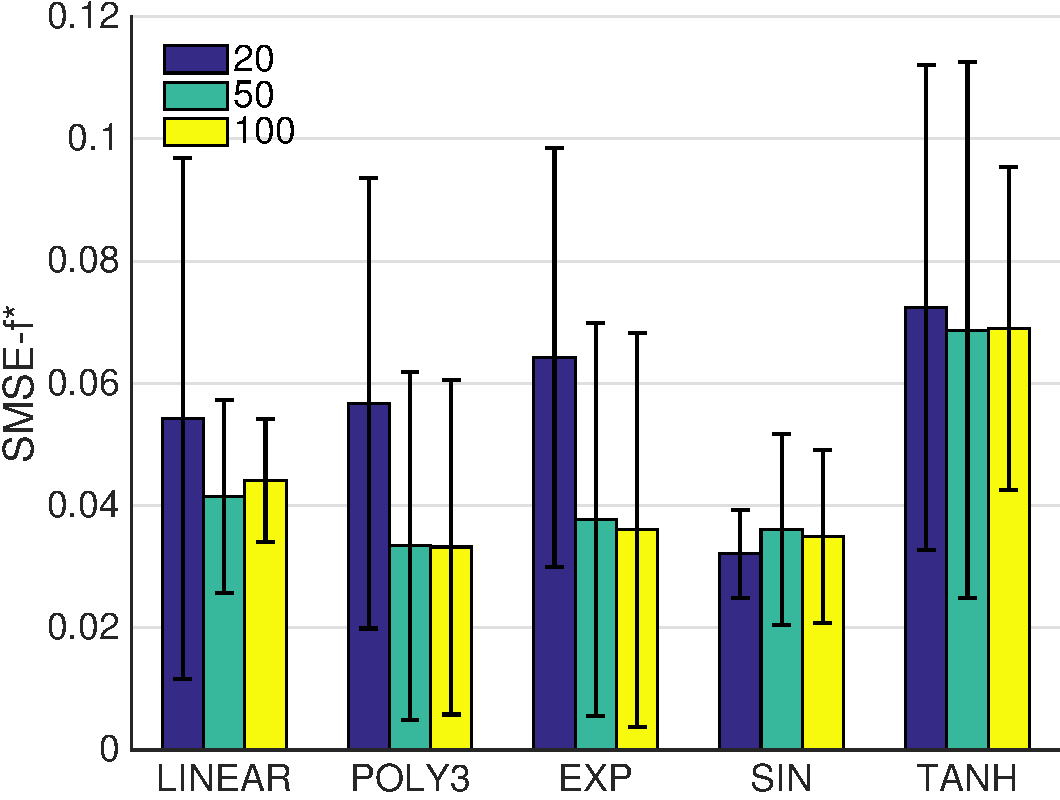
\includegraphics[width=0.31\linewidth]{toyData-EKS-SMSE-fstar} &
\includegraphics[width=0.31\linewidth]{toyData-EKS-NLPD-fstar} &
\includegraphics[width=0.31\linewidth]{toyData-EKS-SMSE-gstar} \\
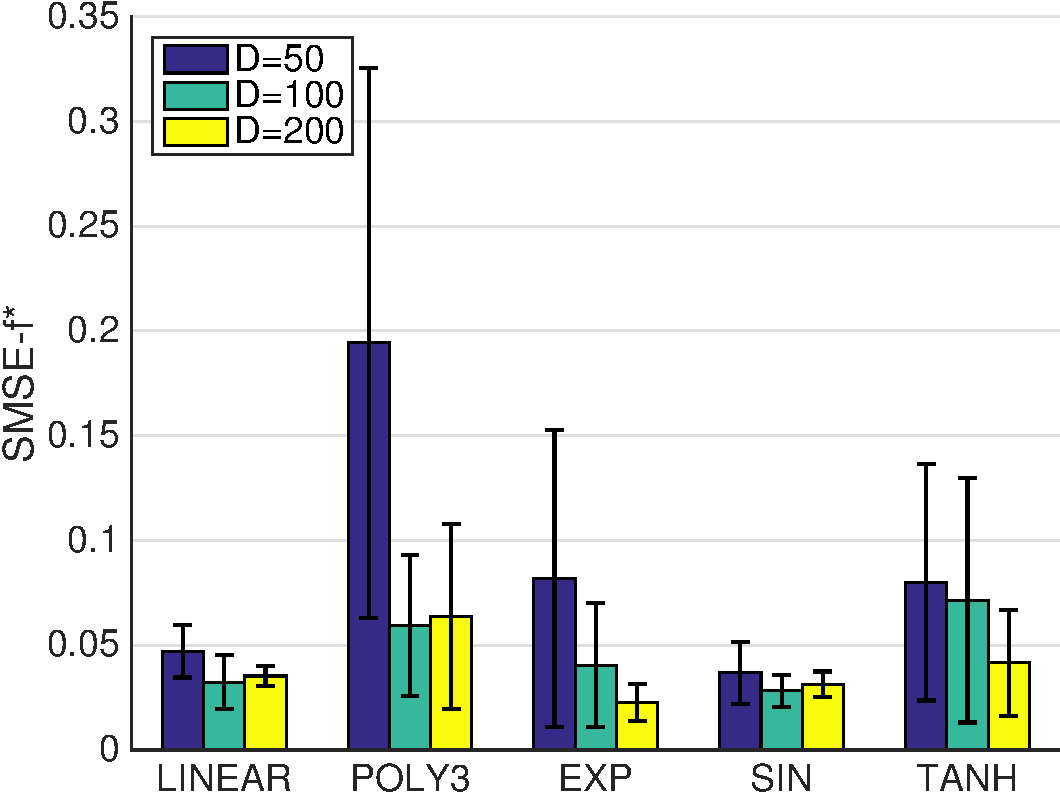
\includegraphics[width=0.31\linewidth]{toyData-UKS-SMSE-fstar} &
\includegraphics[width=0.31\linewidth]{toyData-UKS-NLPD-fstar} &
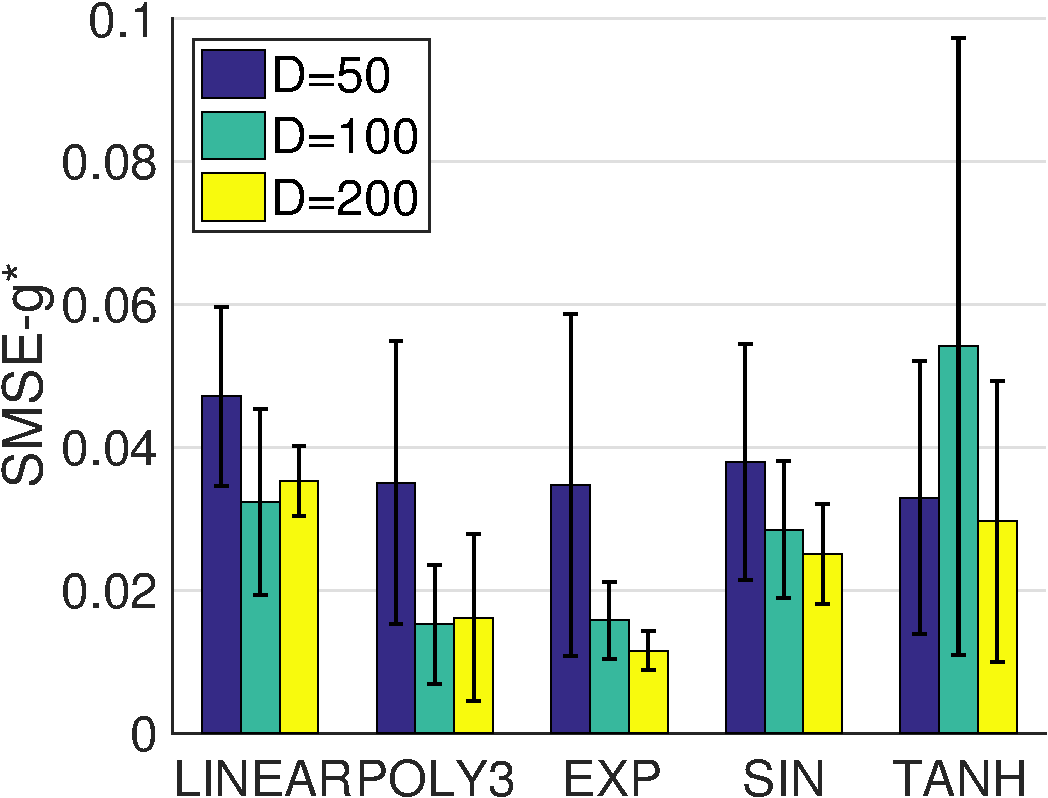
\includegraphics[width=0.31\linewidth]{toyData-UKS-SMSE-gstar} \\
\end{tabular}
\caption{The performance of the \eks (top) and \uks (bottom) as a function of the number of features used. }
\end{figure*}
